\chapter{Introduction}
% What is hardware offloading?
In 1965, Gordon Moore, co-founder of Intel, stated that for the same footprint, the number of transistors in an integrated circuit should double every two years~\cite{moore1965}.
It became the Moore's law, an empirical prediction that drived innovation for fifty years.
Nowadays, it is reaching its limits, as Intel in delaying the manufacturing of its next-generation processors.

The technological limitation is not the only parameter slowing the development of new ICs.
The second law of Moore states that the cost to design, manufacture and test the new architectures doubles every four years.
This economical growth will eventually collide with the Moore's law, stopping its progression.

The domination of multi-purpose processors is reaching its limits, and even the biggest actors on the market are considering alternatives to the Moore's Law.

\noindent A report of the Natural Resources Defense Council~\cite{nrdc2014} forecasts the US datacenter electricity bill to reach \$13.7 billion by 2020.
As CPUs are largely responsible for the power consumption, it makes their design critical.
A solution is to use a hybrid architecture, combining a general-purpose micro-processor with an integrated circuit configurable on-the-fly.
This is a path Intel is exploring with its new Xeon product line, a processor aimed at servers, that combines a Xeon CPU with an FPGA from Altera\cite{xeon2014}.\newline{}

On a different scale, Altera developed an ARM based SoC FPGA platform, combining an FPGA with an ARM Cortex-A9.
This platform allows an increase of performance, lower power consumption and reduced board size compared with a solution with an FPGA separated from the CPU.
Such architecture is aimed at embedded and low-energy systems, where not only the performance, but also the power consumption matters.
% on its way to expand that market with the merger with Altera~\cite{2015-intel-altera-merger}.







\section{Aim and purpose of this thesis}
The aim of this thesis is to implement various popular cryptographic schemes on the board, and make use of the embedded hardware device to improve the performance and decrease the ressources utilization.
This work will focus on the network security and the impact of hardware offloading of cryptographic operations.
The testing platform will be the SoCFPGA SoCrates from Altera (see figure~\ref{socrates-photo}), embedding an ARM dual-core Cortex-A9 with an Altera Cyclone V.
Its ethernet interface will allow us to set the platform in a networked environment and test network security protocols.


% Altera and Xilinx are trying to push those SoC plateforms to the market to popularize the FPGAs.

% Power is critical nowadays, esapcially in datacenters.
% Several solutions exists: abandonning general purpose processors altogether and turn towards ARM cores, or add an FPGA to the processor for example.
% Intel proposed the latter solution in 2014~\cite{intel-xeon-fpga} and is on its way to expand that market with the merger with Altera~\cite{2015-intel-altera-merger}.

\begin{figure}[ht]
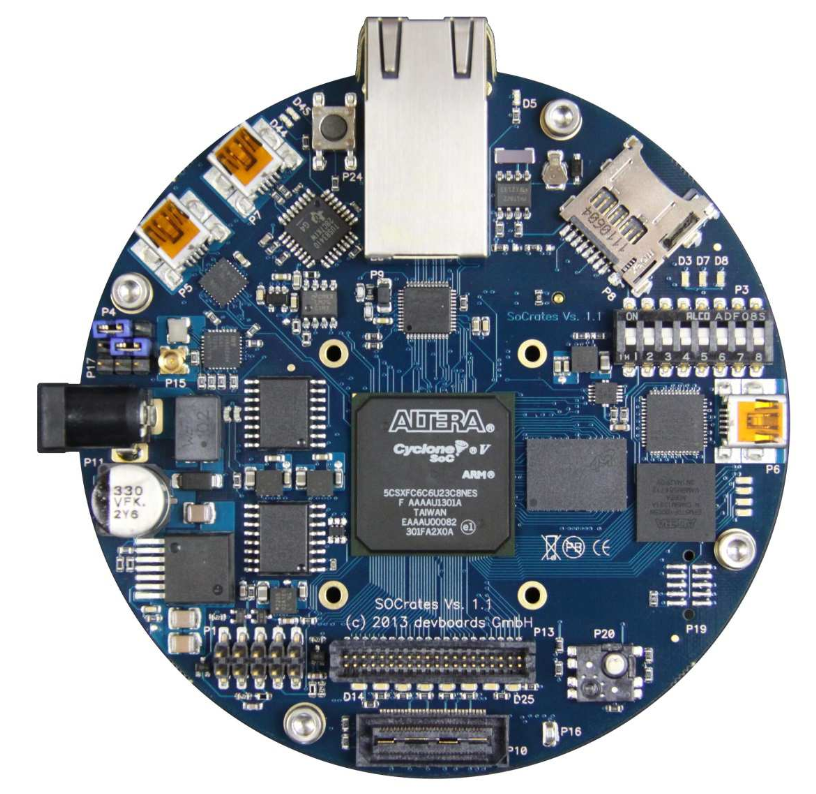
\includegraphics[width=\linewidth]{socrates-photo}
\caption{Altera SoCrates platform}{Combines an ARM Cortex-A9 with an Altera Cyclone V.}
\label{socrates-photo}
\end{figure}





\section{Context}
The work presented in this thesis has been conducted under the supervision of Sébastien Rabou, in Barco Silex' office in Louvain-la-Neuve, between November 2014 and May 2015.\newline{}

% There are diffirent ways to add cryptographic capabilities to an application:
% \begin{itemize}
% 	\item Having the cipher built in.
% 	\item Using a cryptographic library, such as OpenSSL.
% 	\item Using the Linux Crypto API.
% \end{itemize}

In order to make use of the embedded FPGA, two crypto IP cores of Barco Silex will be used: the BA411E~\cite{barco-ba411e} for AES, and the BA414E~\cite{barco-ba414e} for the public key operations.




\section{Structure}
The present document will begin with the technical ground necessary to this work.
After a presentation on how to drive a hardware device from the operating system and details on device driver design, we will address the cryptography.
Only most relevant part of cryptography will be detailed: message digests, symmetric cryptography and more specifically the CBC and GCM modes of operation, and asymmetric cryptography with an accent on RSA and Diffie-Hellman.

The next chapter will present the implementation methods for the protocols theoretically introduced.
Four applications are considered: OpenVPN, OpenSSH, OpenSSL and Strongswan.

Before presenting the results of those implementations, the tests protocols will be discussed and the platforms introduced.
Three tests will be undertaken: TLS connections, latency and file transfer.

The results will address those three tests for different implementations, and the impact of hardware offloading will be analyzed and compared.

Finally, some future works and directions that the project could take are gathered in the last chapter, followed by a concluding word.